\documentclass{article}

%%%%%%%%%%%%%%%%%%%%%%%%%%%%%%%%%%%%%%%%%
% Lachaise Assignment
% Structure Specification File
% Version 1.0 (26/6/2018)
%
% This template originates from:
% http://www.LaTeXTemplates.com
%
% Authors:
% Marion Lachaise & François Févotte
% Vel (vel@LaTeXTemplates.com)
%
% License:
% CC BY-NC-SA 3.0 (http://creativecommons.org/licenses/by-nc-sa/3.0/)
% 
%%%%%%%%%%%%%%%%%%%%%%%%%%%%%%%%%%%%%%%%%

%----------------------------------------------------------------------------------------
%	PACKAGES AND OTHER DOCUMENT CONFIGURATIONS
%----------------------------------------------------------------------------------------

\usepackage{amsmath,amsfonts,stmaryrd,amssymb} % Math packages

\usepackage{enumerate} % Custom item numbers for enumerations

\usepackage{url}

\usepackage[ruled]{algorithm2e} % Algorithms

\usepackage[framemethod=tikz]{mdframed} % Allows defining custom boxed/framed environments

\usepackage{listings} % File listings, with syntax highlighting
\lstset{
	basicstyle=\ttfamily, % Typeset listings in monospace font
}

%----------------------------------------------------------------------------------------
%	DOCUMENT MARGINS
%----------------------------------------------------------------------------------------

\usepackage{geometry} % Required for adjusting page dimensions and margins

\geometry{
	paper=a4paper, % Paper size, change to letterpaper for US letter size
	top=1.5cm, % Top margin
	bottom=2.5cm, % Bottom margin
	left=2.4cm, % Left margin
	right=2.4cm, % Right margin
	headheight=10pt, % Header height
	footskip=1.5cm, % Space from the bottom margin to the baseline of the footer
	headsep=1cm, % Space from the top margin to the baseline of the header
	% showframe, % Uncomment to show how the type block is set on the page
}

%----------------------------------------------------------------------------------------
%	FONTS
%----------------------------------------------------------------------------------------

\usepackage[utf8]{inputenc} % Required for inputting international characters
\usepackage[T1]{fontenc} % Output font encoding for international characters

% \usepackage{XCharter} % Use the XCharter fonts\usepackage{XCharter} % Use the XCharter fonts

%----------------------------------------------------------------------------------------
%	COMMAND LINE ENVIRONMENT
%----------------------------------------------------------------------------------------

% Usage:
% \begin{commandline}
%	\begin{verbatim}
%		$ ls
%		
%		Applications	Desktop	...
%	\end{verbatim}
% \end{commandline}

\mdfdefinestyle{commandline}{
	leftmargin=10pt,
	rightmargin=10pt,
	innerleftmargin=15pt,
	middlelinecolor=black!50!white,
	middlelinewidth=2pt,
	frametitlerule=false,
	backgroundcolor=black!5!white,
	frametitle={Command Line},
	frametitlefont={\normalfont\sffamily\color{white}\hspace{-1em}},
	frametitlebackgroundcolor=black!50!white,
	nobreak,
}

% Define a custom environment for command-line snapshots
\newenvironment{commandline}{
	\medskip
	\begin{mdframed}[style=commandline]
}{
	\end{mdframed}
	\medskip
}

%----------------------------------------------------------------------------------------
%	FILE CONTENTS ENVIRONMENT
%----------------------------------------------------------------------------------------

% Usage:
% \begin{file}[optional filename, defaults to "File"]
%	File contents, for example, with a listings environment
% \end{file}

\mdfdefinestyle{file}{
	innertopmargin=1.6\baselineskip,
	innerbottommargin=0.8\baselineskip,
	topline=false, bottomline=false,
	leftline=false, rightline=false,
	leftmargin=1cm,
	rightmargin=1cm,
	singleextra={%
		\draw[fill=black!10!white](P)++(0,-1.2em)rectangle(P-|O);
		\node[anchor=north west]
		at(P-|O){\ttfamily\mdfilename};
		%
		\def\l{3em}
		\draw(O-|P)++(-\l,0)--++(\l,\l)--(P)--(P-|O)--(O)--cycle;
		\draw(O-|P)++(-\l,0)--++(0,\l)--++(\l,0);
	},
	nobreak,
}

% Define a custom environment for file contents
\newenvironment{file}[1][File]{ % Set the default filename to "File"
	\medskip
	\newcommand{\mdfilename}{#1}
	\begin{mdframed}[style=file]
}{
	\end{mdframed}
	\medskip
}

%----------------------------------------------------------------------------------------
%	NUMBERED QUESTIONS ENVIRONMENT
%----------------------------------------------------------------------------------------

% Usage:
% \begin{question}[optional title]
%	Question contents
% \end{question}

\mdfdefinestyle{question}{
	innertopmargin=1.2\baselineskip,
	innerbottommargin=0.8\baselineskip,
	roundcorner=5pt,
	nobreak,
	singleextra={%
		\draw(P-|O)node[xshift=1em,anchor=west,fill=white,draw,rounded corners=5pt]{%
		Question \theQuestion\questionTitle};
	},
}

\newcounter{Question} % Stores the current question number that gets iterated with each new question

% Define a custom environment for numbered questions
\newenvironment{question}[1][\unskip]{
	\bigskip
	\stepcounter{Question}
	\newcommand{\questionTitle}{~#1}
	\begin{mdframed}[style=question]
}{
	\end{mdframed}
	\medskip
}

%----------------------------------------------------------------------------------------
%	WARNING TEXT ENVIRONMENT
%----------------------------------------------------------------------------------------

% Usage:
% \begin{warn}[optional title, defaults to "Warning:"]
%	Contents
% \end{warn}

\mdfdefinestyle{warning}{
	topline=false, bottomline=false,
	leftline=false, rightline=false,
	nobreak,
	singleextra={%
		\draw(P-|O)++(-0.5em,0)node(tmp1){};
		\draw(P-|O)++(0.5em,0)node(tmp2){};
		\fill[black,rotate around={45:(P-|O)}](tmp1)rectangle(tmp2);
		\node at(P-|O){\color{white}\scriptsize\bf !};
		\draw[very thick](P-|O)++(0,-1em)--(O);%--(O-|P);
	}
}

% Define a custom environment for warning text
\newenvironment{warn}[1][Warning:]{ % Set the default warning to "Warning:"
	\medskip
	\begin{mdframed}[style=warning]
		\noindent{\textbf{#1}}
}{
	\end{mdframed}
}

%----------------------------------------------------------------------------------------
%	INFORMATION ENVIRONMENT
%----------------------------------------------------------------------------------------

% Usage:
% \begin{info}[optional title, defaults to "Info:"]
% 	contents
% 	\end{info}

\mdfdefinestyle{info}{%
	topline=false, bottomline=false,
	leftline=false, rightline=false,
	nobreak,
	singleextra={%
		\fill[black](P-|O)circle[radius=0.4em];
		\node at(P-|O){\color{white}\scriptsize\bf i};
		\draw[very thick](P-|O)++(0,-0.8em)--(O);%--(O-|P);
	}
}

% Define a custom environment for information
\newenvironment{info}[1][Info:]{ % Set the default title to "Info:"
	\medskip
	\begin{mdframed}[style=info]
		\noindent{\textbf{#1}}
}{
	\end{mdframed}
}

\usepackage{fontspec}
\usepackage{xeCJK}
\usepackage{url}
\usepackage{subfigure}

\setCJKmainfont{SimSun}
\setlength{\parindent}{0em}
\setlength{\parskip}{1em}

\title{Nvidia Jetson TX2 开发板测试报告}

\author{Zhang Yifei(\texttt{yidadaa@qq.com})}

\date{UESTC --- \today}

\begin{document}

\maketitle

\section{环境设置}
Nvidia Jetson TX2 系列开发板提供了大约1.5T Flops的运算能力,可以运行大多数轻量级神经网络。本次测试使用开发板配套的Jetpack套件,测试常见的SLAM系统以及视觉算法在开发板上的表现。
\subsection{解决opencv无法使用\-lopencv\_nonfree的问题}
Jetpack 自带的 Opencv 不支持 nonfree 库,因此就不能使用SIFT/SURF这种专利算法。要使用nonfree库有两种解决解决方法:

Note about SIFT/SURF in the nonfree module: OpenCV4Tegra doesn’t include the opencv\_nonfree package (containing SIFT \& SURF feature detectors) since those algorithms are patented by other companies and therefore anyone using opencv\_nonfree is at risk of liability.

If you need something from the nonfree module, you have 2 options:

\begin{itemize}
    \item Analyze the public OpenCV source code then copy/paste the parts of the nonfree module that you want (eg: SURF feature detector) from OpenCV into your own project. You will have the CPU optimizations of OpenCV4Tegra for most of your code and will have the GPU module and will have the non-optimized patented code that you need from the nonfree package such as SURF. So this option gives full performance (for everything except the nonfree code) but is tedious.
    \item Ignore OpenCV4Tegra, and instead, download \& build public OpenCV (by following the instructions below for natively compiling the OpenCV library from source). You will still have the GPU module but not any CPU optimizations, but you won’t need to spend time ripping out parts of the OpenCV non-free module code. So this option is easiest but produces slower code if you are running most of your code on CPU.
\end{itemize}

并且 libopencv4tegra 是2.4版的opencv,要使用3.0+版本的还是得自己编译opencv才行。(缺点是自己编译的opencv没有CPU优化)。

\subsection{开启被屏蔽的2块CPU并设置为最大频率}
使用位于home目录的tegrastats命令可以查看TX-2的使用情况:
\begin{lstlisting}
    $ ~/tegrastats
    RAM 1282/7854MB (lfb 1x256kB)
    cpu [21%@2035,off,off,15%@2035,17%@2035,15%@2035]
\end{lstlisting}
开启被屏蔽的两颗CPU:
\begin{lstlisting}
    $ sudo su
    $ echo 1 > /sys/devices/system/cpu/cpu1/online
    $ echo 1 > /sys/devices/system/cpu/cpu2/online    
\end{lstlisting}
使用以下命令开启最大频率:
\begin{lstlisting}
    ~/jetson_clocks.sh
\end{lstlisting}
再次查看CPU情况:
\begin{lstlisting}
    $ ~/tegrastats
    RAM 979/7854MB (lfb 1545x4MB)
    cpu [0%@2035,0%@2419,0%@2419,0%@2035,0%@2035,0%@2035]
\end{lstlisting}
同时由于频率提升,可以观察到开发板风扇开始转动。

\section{测试SLAM系统}
\subsection{ORB-SLAM}
ORB-SLAM 是西班牙 Zaragoza 大学的 Raúl Mur-Arta 编写的视觉 SLAM 系统。 它是一个完整的 SLAM 系统,包括视觉里程计、跟踪、回环检测,是一种完全基于稀疏特征点的单目 SLAM 系统,其核心是使用 ORB (Orinted FAST and BRIEF) 作为整个视觉 SLAM 中的核心特征。
\begin{figure*}[h]
    \centering
    \subfigure[]{
        \begin{minipage}[t]{0.45\linewidth}
            \centering
            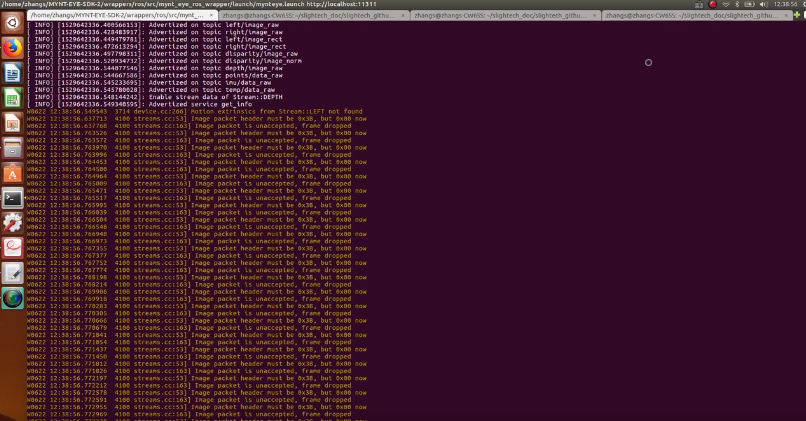
\includegraphics[width=\textwidth]{./orb-slam.png}
        \end{minipage}
    }
    \subfigure[]{
        \begin{minipage}[t]{0.45\linewidth}
            \centering
            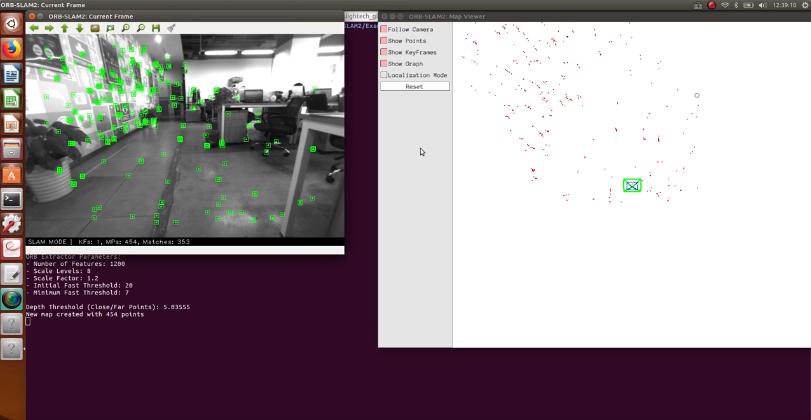
\includegraphics[width=\textwidth]{./orb-slam-1.png}
        \end{minipage}
    }
    \caption{ORB-SLAM测试截图}
\end{figure*}

在测试过程中,使用720P分辨率的图像作为输入,处理速度可以稳定在30FPS,基本可以达到可用级别。

\subsection{OKVIS}
OKVIS是由 Stefan Leutenegge 等人提出的基于双目+惯导的视觉里程计,属于 VIO (Visual Inertial Odometry) 。
\begin{figure*}[h]
    \centering
    \subfigure[]{
        \begin{minipage}[t]{0.45\linewidth}
            \centering
            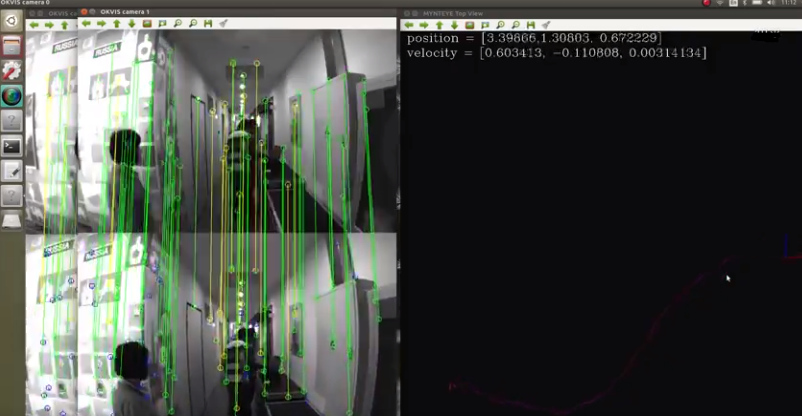
\includegraphics[width=\textwidth]{./okvis.png}
        \end{minipage}
    }
    \subfigure[]{
        \begin{minipage}[t]{0.45\linewidth}
            \centering
            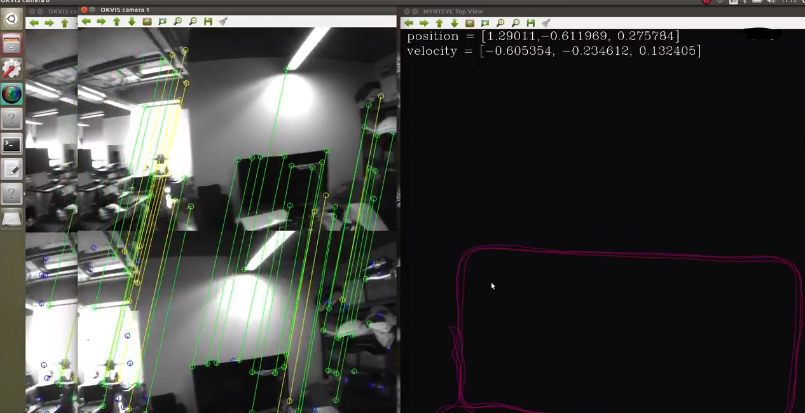
\includegraphics[width=\textwidth]{./okvis-1.png}
        \end{minipage}
    }
    \caption{ORB-SLAM测试截图}
\end{figure*}
OKVIS系统由于需要将双目图像与IMU数据同步,需要大量运算,在720P视频下,可以达到15FPS的速度,在不影响使用的情况下,将分辨率降至480P可以使帧率提升到27FPS左右,基本达到可用水平。

\section{总结}
本次测试使用两个机器人导航中常用的SLAM算法,Jetson TX2 基本可以胜任此类算法的运行任务,可以在此平台上进一步开发用于机器人导航或环境建图的边缘端计算平台。

\end{document}
